\section{Optimised Logistics}

\begin{marginfigure}
\checkoddpage \ifoddpage \forcerectofloat \else \forceversofloat \fi
\centering
 \frame{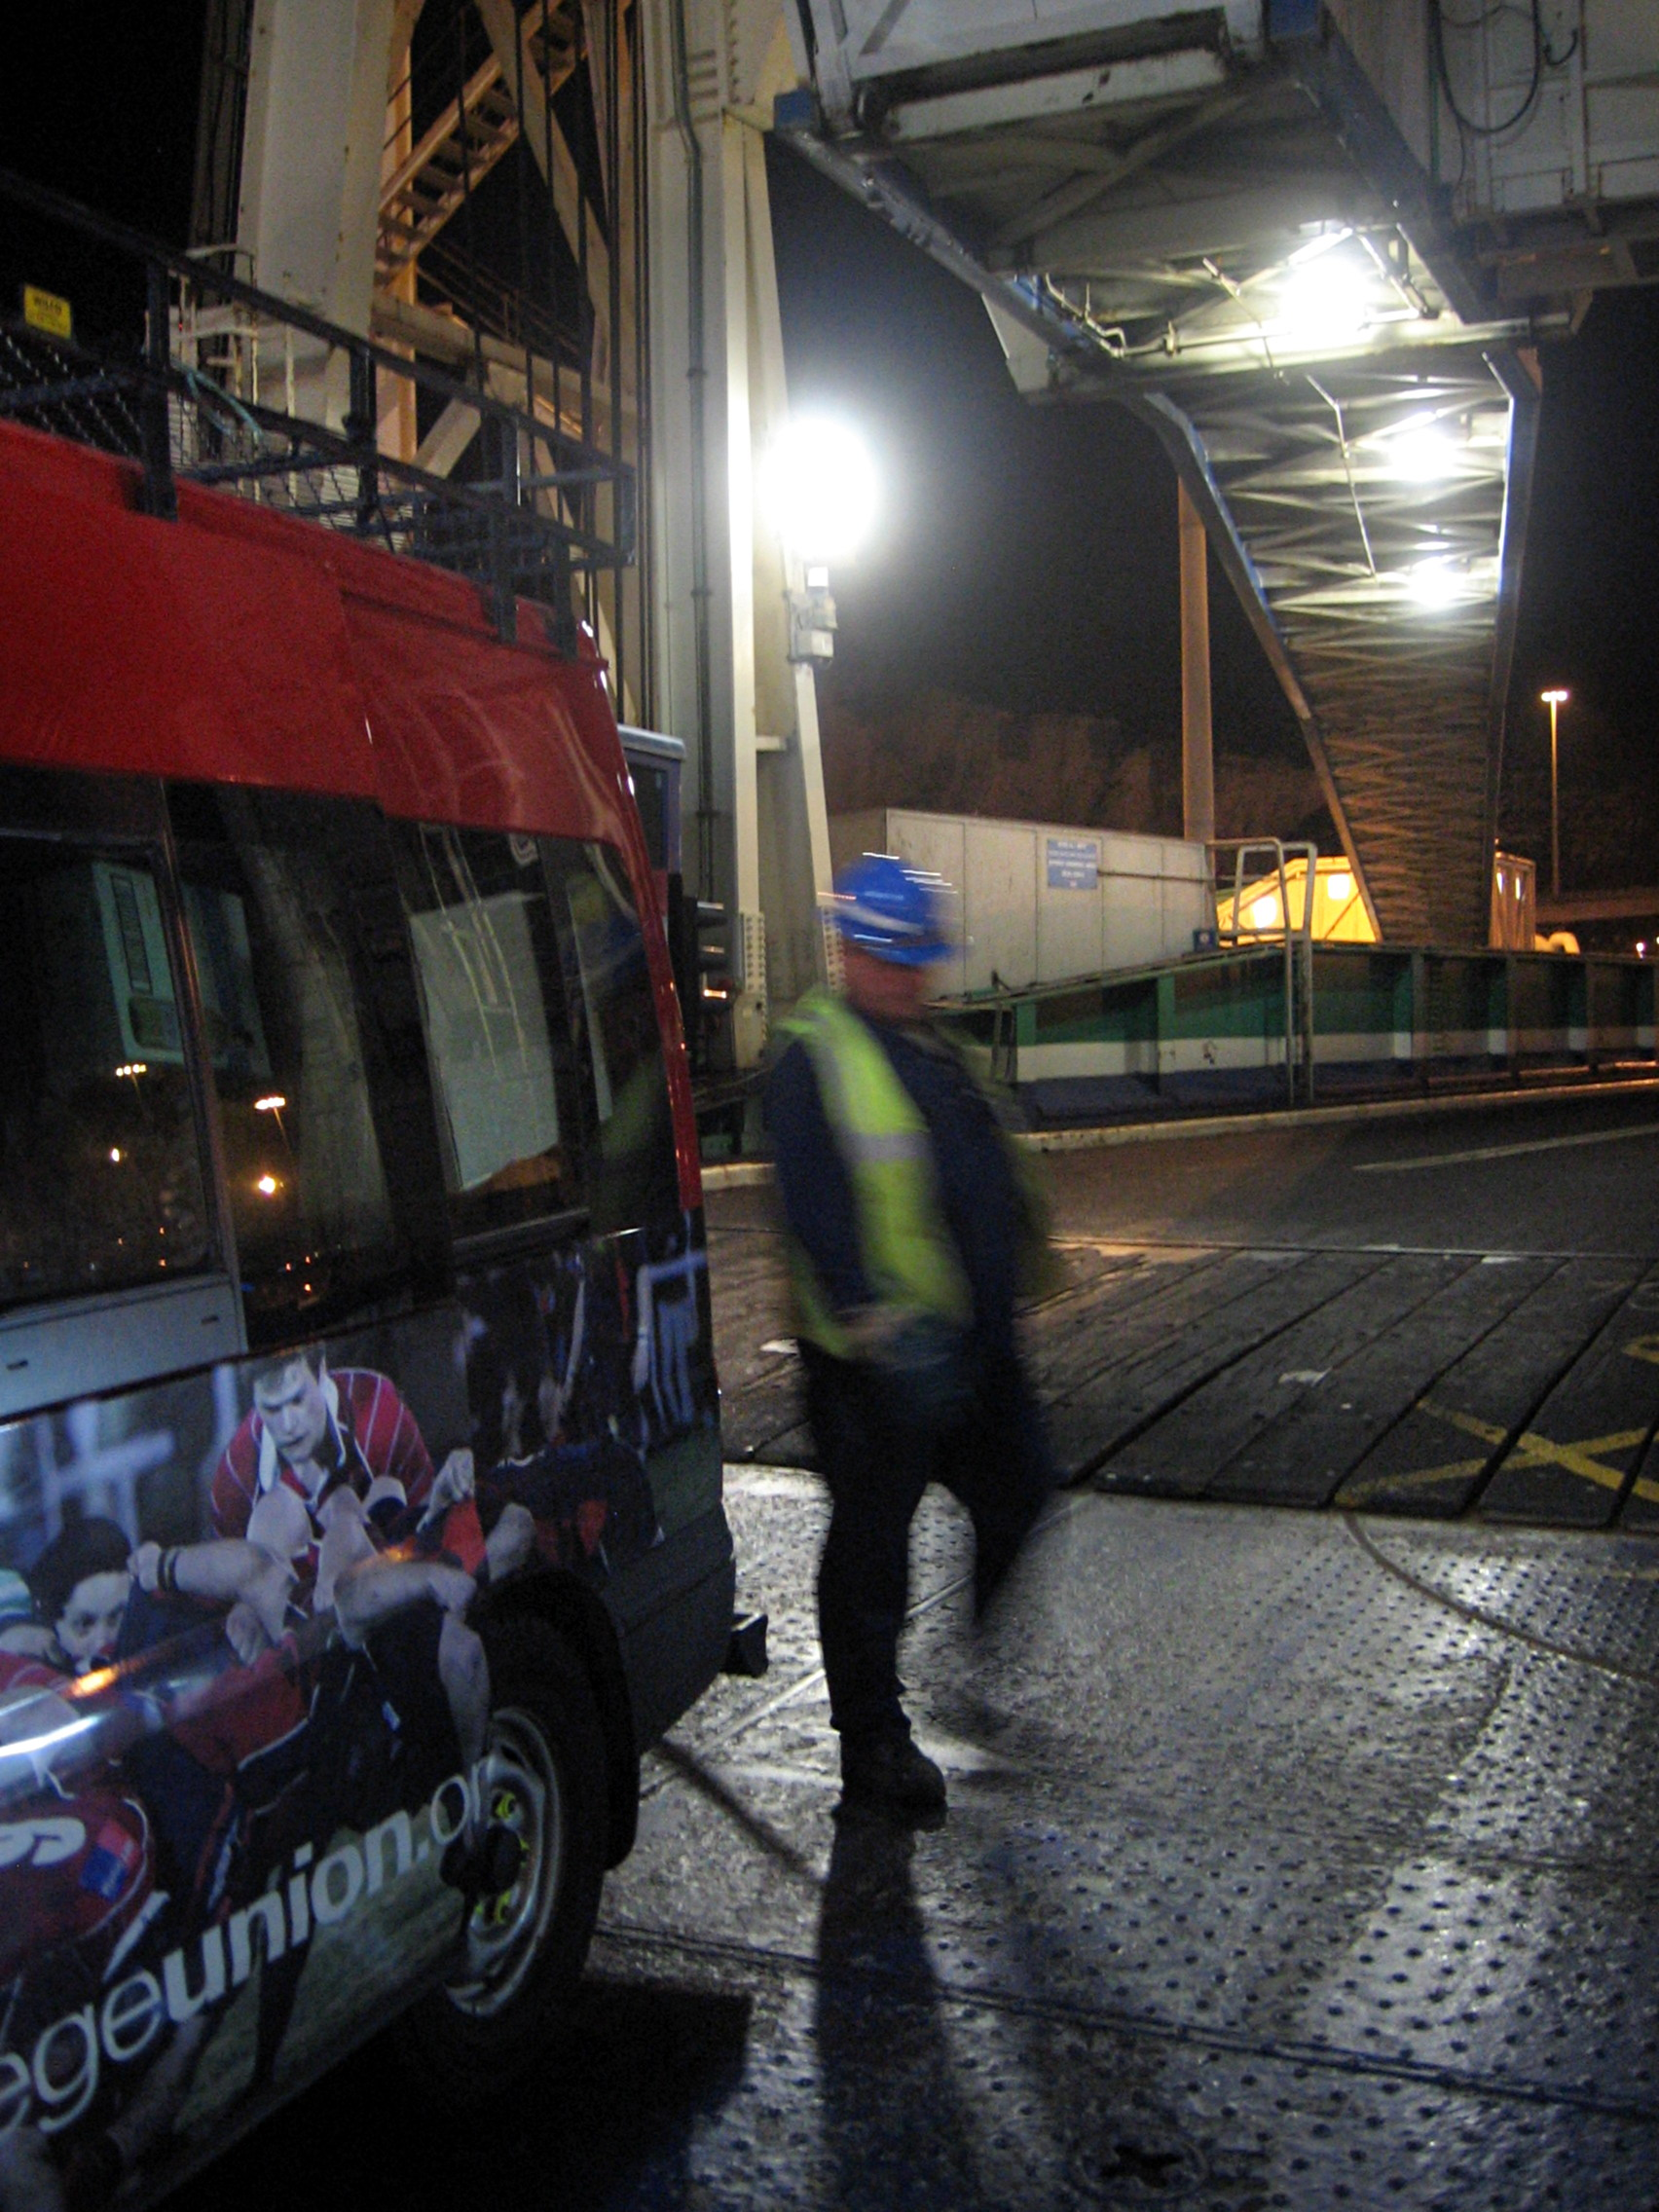
\includegraphics[width=\linewidth]{2009/logistics/2009-07-25-01.32.29 - Jarvist Frost - Canon Powershot A520 - Loading onto the ferry in Dover--orig.jpg}} 
 \caption{Catching the ferry in \protect\passage[town]{Dover} at 1:32AM. \pic{Jarvist Frost}}
 \label{ferry 2009}
\end{marginfigure}

Our logistics have been heavily optimised over the last ten years of
returning to this same plateau. The main difficulty is in lifting (this
year purely through manpower) our food and equipment from \passage[town]{Tolminske
Ravne} (where we can drive to) at 912 m to the bivouac in a shakehole
under a rockbridge at 1860 m (the \passage{Bivi}).

A further optimisation that we have carried out the last few years is in
using the derig carries at the end of the previous year to bring up
sufficient non-perishable foods (rice, pasta etc.) to eat during the
first half of the expedition in the present year. This way, caving can
start fully after just two or three carries per team member, rather than
the more traditional `week of carries' that characterised the old
six-week expeditions!

A further refinement was leaving from \passage[town]{London} with the Minibus on Friday
night. Though rather harsh on the drivers, this meant that we arrived in
\passage[town]{Tolmin} on Saturday just in time for a well-earned proper meal and a full
night of sleep before an alpine start. Up shortly after dawn, we had
managed to acquire the necessary petrol for cooking and other locally
bought fresh food.

\begin{marginfigure}
\checkoddpage \ifoddpage \forcerectofloat \else \forceversofloat \fi
\centering
 \frame{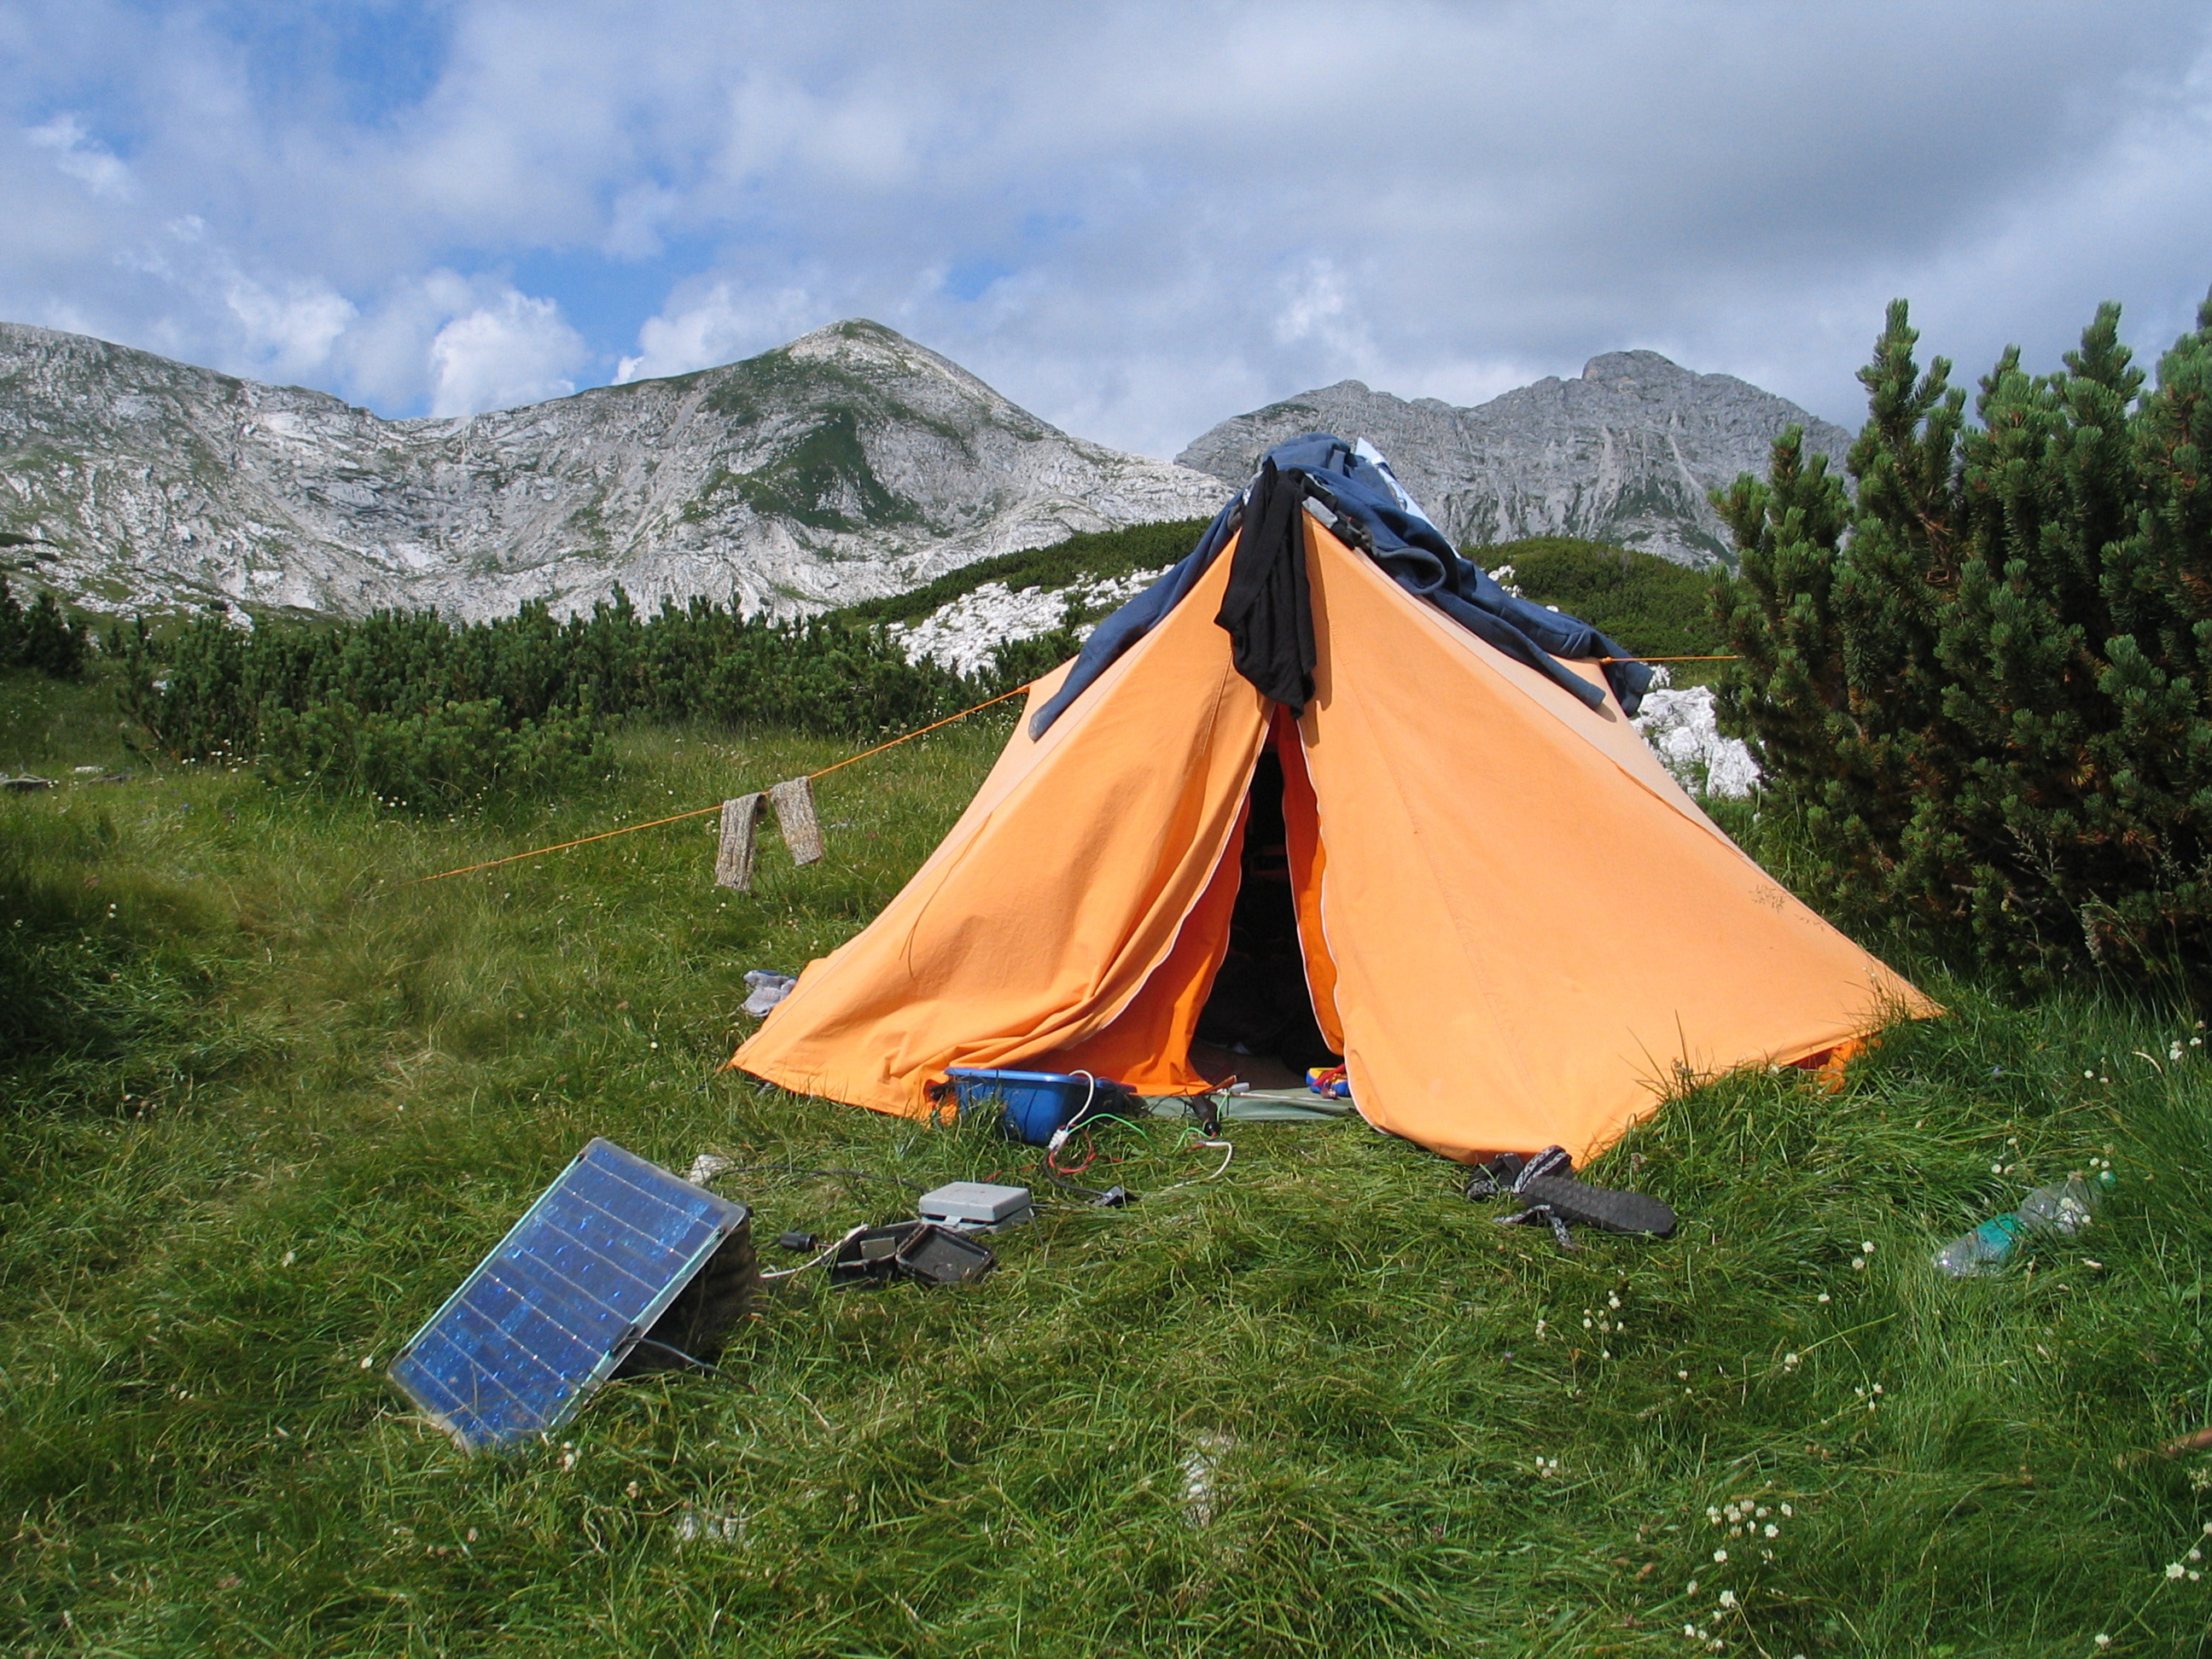
\includegraphics[width=\linewidth]{2009/logistics/2009-08-07-13.23.46 - Jarvist Frost - Canon Powershot G5 - F10 on the plateau with solar panel and drying caving gear--orig.jpg}} 
 \caption{Putting the solar panel outside a tent to run as 'charging station', rather than relying on people fetching the battery and panel from the \passage{Bivi} every morning, makes a lot of sense. \pic{Jarvist Frost}}
 \label{panel F10}
\end{marginfigure}

Our drill batteries were charged on mains power down in the village and
then carried up, but power for rechargeable lights, survey laptop, MP3
player \& underground camp speakers were all provided for by a small
photovoltaic panel placed next to a tent.
\name{Jarvist Frost}




\begin{quote}
    All men dream: but not equally\\
Those who dream by night in the dusty\\
recesses of their minds wake in the day\\
to find that it was vanity: but the dreamers\\
of the day are dangerous men, for they may\\
act their dreams with open eyes, to make it\\
possible.
\end{quote}
\textbf{T.E. Lawrence, The Seven Pillars of Wisdom}


\begin{pagefigure}
\checkoddpage \ifoddpage \forcerectofloat \else \forceversofloat \fi
\frame{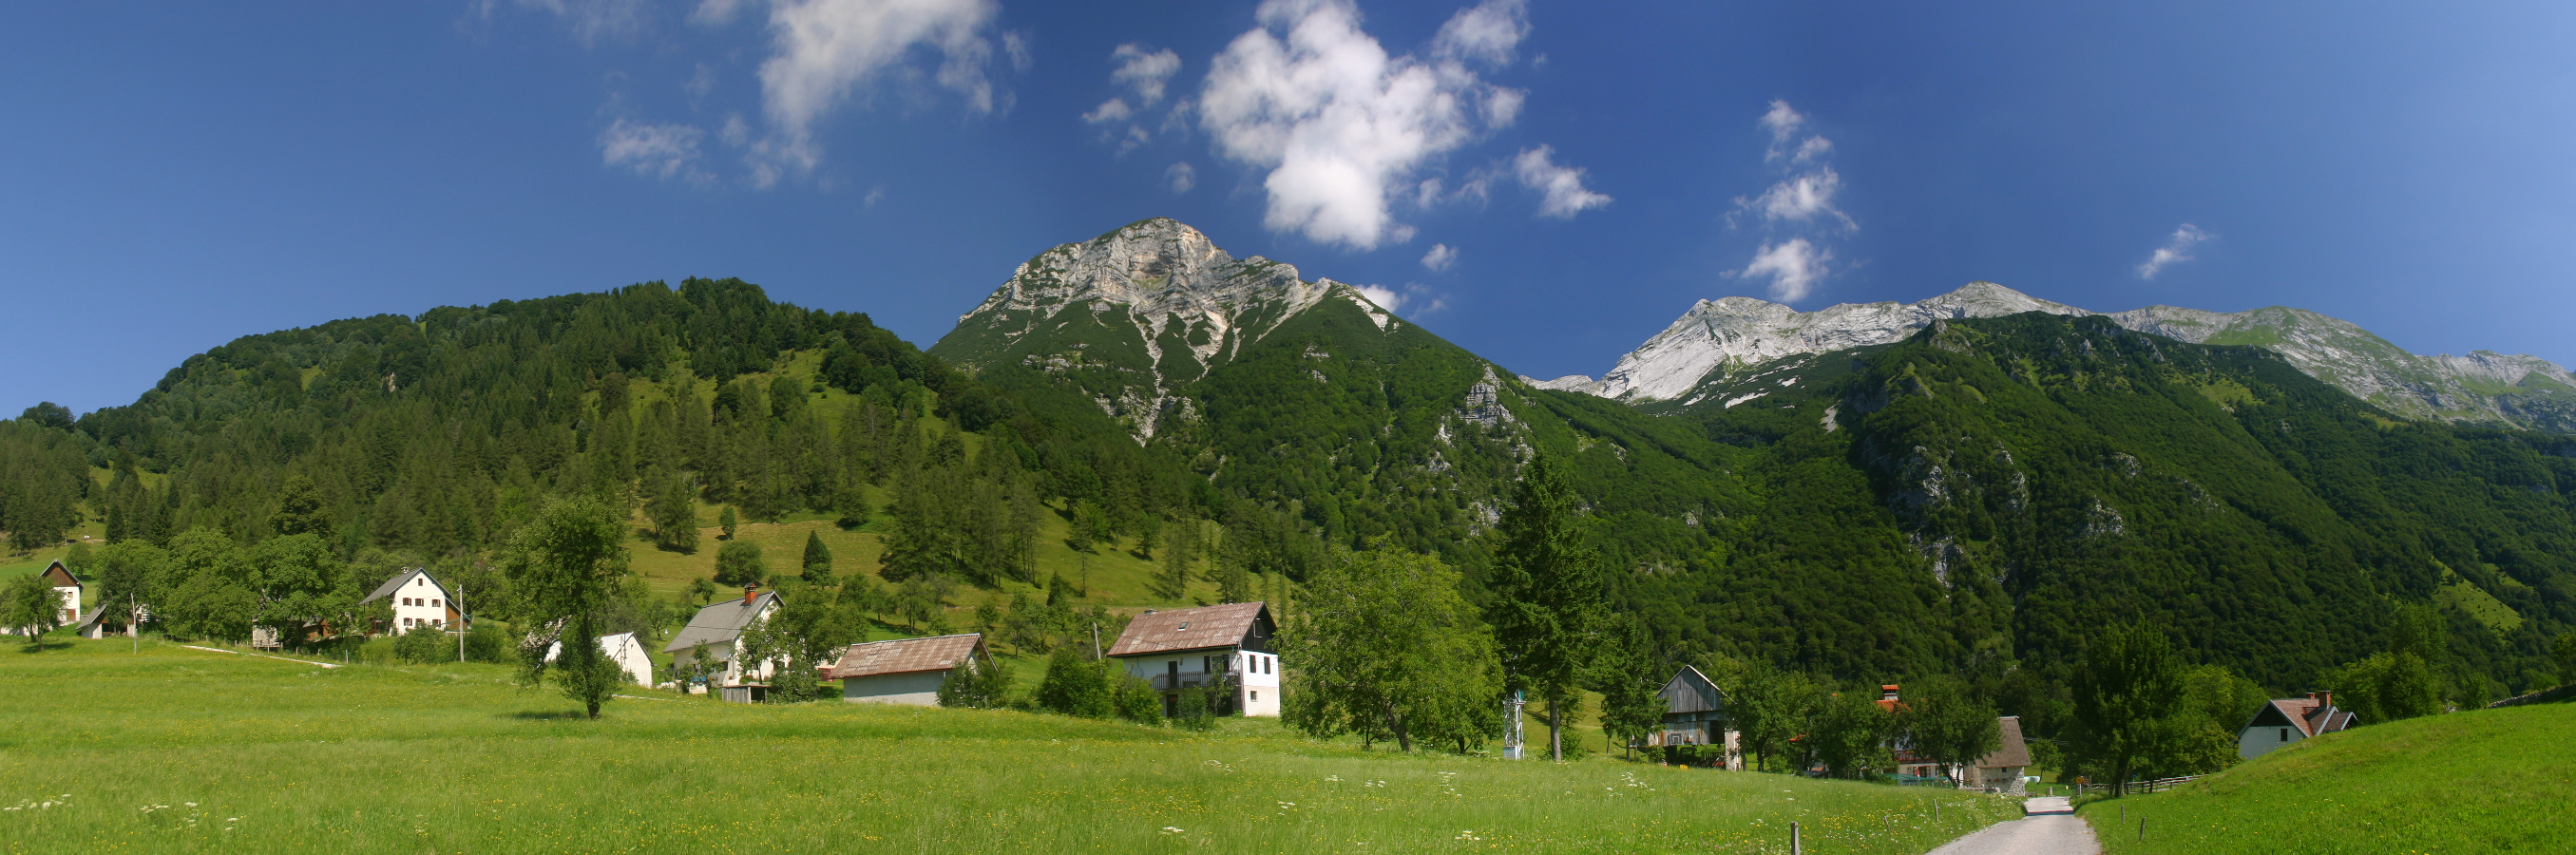
\includegraphics[width=\linewidth]{2009/planning/2009-07-27-15.56.43 - Tharatorn Supasiti - Ravne 2 - IMG_5317-5320-ravne.jpg}}
\caption{The hamlet of \protect\passage{Tolminske Ravne} on July 27\(^{th}\) 2009. \pic{Tharatorn Supasiti}}
\end{pagefigure}